\chapter{Meteorological Instrumentation for real-time operation 
}
%\\ \color{green} POST PUBLIC REVIEW VERSION\color{black}} 
    \label{ch:instrumentation}
{\color{magenta}{Contributing author: COM, JB}}

\noindent
\begin{tcolorbox}
\parbox{\textwidth}{
\emph{\textbf{Key Points}\\
In this section currently applied as well as instrumentation that is under development is being described... 
}}
\end{tcolorbox}

The purpose of meteorological measurements as supplement to the power measurements at wind and solar plants is to provide a measure of the resource and weather situation at the specific location and any given time. This information should not only come from an obligation to wind and solar plant operators defined in the technical requirements of system operators, but has equally much become a tool to optimise the operation of wind turbines and solar plants by the operators.

For both the system operator and the plant operator, these measurements are an independent signal at the plant location that can warn about critical weather and provide an indication on whether the wind turbines and solar panels work at their expected performance level. For the transmission system operator, such measurements can additionally be used for situational awareness of the weather in the control area that may affect the transmission lines. They also provide a second means of verification, whether the power signal at a given wind or solar plant is malfunctioning in situations that may be critical in terms of grid operation.
Meteorological centres have also shown an interest in these data for the data assimilation of the numerical weather prediction models (e.g.\citep{Marquis2012,EWeLINE2011}) that typically lack observational information at hub heights. 

One of the most important findings so far has been that the quality of data provided is the most essential issue to be solved in order to gain higher quality forecasts with such measurements. In fact, it has been identified that if there is no specific effort put into standardisation of requirements in the power industry, the benefits cannot be achieved.

The following is a list of typical instrumentation used for wind and solar projects that will be subject for this recommended practice guideline and recommendations made in how to setup these instruments and which implications the use of the various instruments have on data quality and usability in the operational real-time context in the energy industry.

\section{Instrumentation for Wind projects}\label{sec:wind_instrumentation}

Typical instrumentation for meteorological measurements in wind power context are divided into two categories: 

%\subsubsection{Components of a wind measurement systems} moved from chapter 4
%A measurement system for wind projects maybe built from the following components:
\begin{itemize}
    \item Met mast
        \begin{enumerate}
            \vspace{-0.2cm}\item Lattice masts
            \vspace{-0.2cm}\item Telescope masts
        \end{enumerate}
    \item Steel cabinet
        \begin{enumerate}
            \vspace{-0.2cm}\item Data logger
            \vspace{-0.2cm}\item Communication system
           \vspace{-0.2cm} \item Components for the power supply
            \vspace{-0.2cm}\item Additional system components
                \begin{itemize}
                        \vspace{-0.2cm}\item Anemometers
                       \vspace{-0.2cm} \item Wind vanes
                       \vspace{-0.2cm} \item Temperature humidity sensors
                        \vspace{-0.2cm}\item Air pressure sensors
                         \vspace{-0.2cm}\item hygrometer sensors
                        \vspace{-0.2cm}\item precipitation sensors rain gauges   
                \end{itemize}
        \end{enumerate}
    \item Remote Sensing Systems
        \begin{enumerate}
            \item LiDAR
            \begin{itemize}
                    \item Wind Profiling LiDAR
                    \item Scanning LiDAR (Long-Range and short-range)
                    \item Nacelle-based LiDAR
                \end{itemize}
            \item SoDAR
        \end{enumerate}
\end{itemize}



Not so common instrumentation or additional instrumentation for wind farms are:
\begin{itemize}
    \item Microwave Radiometers (measures energy emitted at sub-millimetre-to-centimetre wavelengths at frequencies of 1–1000GHz)  
    \item Ceilometer (light source to determine the height of a cloud base. Ceilometers can also be used to measure the aerosol)
    \item Microbarographs (measures atmospheric pressure)
\end{itemize}

These instrumentation are more commonly used in research measurement campaigns and in meteorological projects. Literature on these types such as microwave radiometers are described by e.g.  \cite{Ulaby1982,Matzler2006}, for ceilometers by \cite{Morris2016}, or microbarographs by \cite{Monserrat1992}.



%\section{Meteorological masts for wind farms} \label{subsec:meteorological_masts}

Meteorological mast are still the most commonly used measurement instrumentation for the planning phase and operation of wind farms. An example is shown in Figure \ref{fig:met_mast}. 


\begin{figure}[h!]
\center
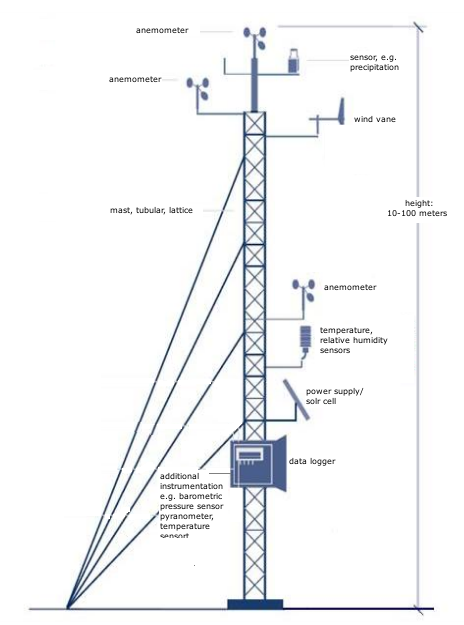
\includegraphics[width=0.5\textwidth]{figures/typical_met_mast.png}
\caption{Example of a typical met mast with various instrumentation, data logger, power supply and wiring. Typical instrumentation are cup anemometers or sonic anemometers, wind vanes, temperature, pressure and air density sensors, pyranometers and precipitation and humidity  sensors.}
\label{fig:met_mast}
\end{figure}

%%%% repetition -- see section \label{sec:wind_instrumentation}
%Typically, these met masts have the following instrumentation attached: 
%\begin{itemize}
%     \vspace{-0.2cm}\item wind vanes
%     \vspace{-0.2cm}\item cup and/or (ultra) sonic anemometers
%     \vspace{-0.2cm}\item temperature sensors
%     \vspace{-0.2cm}\item pressure sensors
%     \vspace{-0.2cm}\item humidity sensors and rain gauges
%\end{itemize}

\iffalse
For resource or site assessment in the planning phase of a wind farm an IEC standard exists \citep{iec17025-2005E} with an updated version 2 (IEC 61400-12-2:2013), that specifies which tests and what kind of criteria the instrumentation has to fulfil when used for the required tests to be carried out. The IEC 61400-12-2:2013 rules contain the following items:
\begin{itemize}
    \item Extreme winds
    \item Shear of vertical wind profile
    \item Flow inclination
    \item Background turbulence
    \item Wake turbulence
    \item Wind-speed distribution
\end{itemize}

The results of these tests have to be within a pre-defined range to be acceptable. In Appendix F of the 61400-12-1:2005 "Cup anemometer calibration procedure" the calibration of the instruments for measuring wind are specified \cite{iec61400-12-1-2005}.\\


MEASNET (MEASuring NETwork), the "international network for harmonised and recognized measurements in wind energy" has defined so called "Round Robin rules" for calibration of cup anemometers for wind energy \cite{measnet2009}, which are widely used. MEASNET has also  published a number of guidelines regarding instrument calibration and measurement campaigns for the wind industry within the EU project ACCUWIND (\cite{Dahlberg2006,Pedersen2006, Eecen2006}. Lee [2008] found a way of calibrating wind direction sensors with an optical camera.

The Annex D in IEC 61400-12-1:2005 standard states that the "implicit assumption of the method of this standard is that the 10 min mean power yield from a wind turbine is fully explained by the simultaneous 10 min mean wind speed measured at hub height, and the air density" [IEC, 2005, Annex D, Table D.1] and describes the associated measurement uncertainty evaluation principles.  In this respect, the standard refers to the "ISO Guide to the expression of Uncertainty in Measurements" \citep{jcgm2008,jcgm2009,jcgm2012} and its 2 supplements [\citep{jcgm2008a,jcgm2011} from the Joint Committee for Guides in Meteorology (JCGM), where there are two types of measurement uncertainty that are to be accounted for in any standardised measurement taking: 
\begin{enumerate}
    \item systematic errors, which are also known as measurement bias, often associated with offsets of the measured quantity
    \item random errors, which are associated with the fact that 2 measurements of the same quantity are seldom the same
\end{enumerate}

In section 3.1.2 of the guide, \citep{jcgm2008,jcgm2011} it is stated that "the result of a measurement .. is only an approximation or estimate .. of the value of the measurand and thus is complete only when accompanied by a statement of the uncertainty ... of that estimate". Considering this definition, all measurements should ideally have an uncertainty term associated with it. This is impractical in real-time operations, where the value of the measurements lies in the availability of the data at a given time. Therefore, it is unrealistic to request uncertainty measures. However, it could be a standing data value that is determined at the setup of the instrument and provided as part of the standing data. In that way, the instrument specific uncertainty could be accounted for in the handling of measurements.\\ 

The alternative is to carry out an uncertainty estimation with e.g. the Monte-Carlo method described in \citep{jcgm2011} pp23-33) or a mean uncertainty value must be added to raw measurements, as applied by Pinson and Hagedorn in an experiment over Ireland and Denmark with wind measurements from standard met masts [Pinson and Hagedorn, 2012 p7]. If a more standardised technical requirement is desirable, the JCGM guides offer a valuable general source, also applied in meteorology and oceanography. In that way, a harmonisation of "best practices" with these directly related real-time disciplines can be achieved. In fact, the guides do not only consider the measurand as a physical quantity, but also provide guidance to the conceptual design and the theoretical analysis of measurements and methods. 

In the introduction to the Guide [JCGM, 2009], it is stated that “..the principles of this Guide are intended to be applicable to a broad spectrum of measurements”, including those required for:
\begin{itemize}
   \item maintaining quality control and quality assurance in production
   \item complying with and enforcing laws and regulations
   \item calibrating standards and instruments and performing tests throughout a national 
   \item measurement system in order to achieve tractability to national standards developing, maintaining, and comparing international and national physical reference standards, including reference materials 
\end{itemize}

To summarise, the handling and integration of wind power into the electric grid is an equally important step to harness the full potential of the energy resource in an efficient and environmentally friendly way. 


This requires that measurements are trustworthy and maintained to a quality that allows for their use in forecasting tools in order to produce high quality forecasts and thereby reduce the need of reserves. These guides in combination with the IEC 61400-1 standard would provide a good foundation for any grid code technical requirement specifications. 
\fi 

\subsection{Remote Sensing Instrumentation for wind farms {\color{magenta}{Needs more shortening... }}{\color{blue}{authors: COM, IW}}}\label{sec:remote-sensing}

%An IEA Wind Task 32 Publication
%A Review of Guidance for Using Ground-Based VerticallyProfiling Wind Lidar For Wind Resource Assessment
%https://zenodo.org/record/3862384

%[1] IEA Wind. Ground-Based Vertically-Profiling Remote Sensing For Wind Resource Assessment. Recommended Practice RP 15. International Energy Agency TCP Wind, Jan. 2013. URL: https://github.com/IEA-Wind-Task-32/RP15-Ground - Based -Remote - Sensing - for - Wind - Resource -Assessment/releases/tag/1.0.
%[2] MEASNET. Evaluation of site-specific wind conditions V2.0. Procedure. MEASNET, Apr. 2016. URL: http://www.measnet .com/wp-content/uploads/2016/05/MeasnetSiteAssessment V2.0.pdf.
%[3] IEC. Wind turbines - Part 12-1: Power performance measurements of electricity producing wind turbines, Edition 2.0. Standard 61400-12-1:2017. International Electrotechnical Commission, Mar. 2017.
%[4] A. Clifton et al. Remote Sensing of Complex Flows by Doppler Wind Lidar: Issues and Preliminary Recommendations.Tech. rep. NREL/TP-5000-64634. NREL, 2015. URL: http://www.nrel.gov/docs/fy16osti/64634.pdf.
%[5] A. Clifton et al. ‘IEA Wind Task 32: Wind Lidar Identifying and Mitigating Barriers to the Adoption of Wind Lidar’. In: Remote Sensing 10.3 (Mar. 2018). DOI:10.3390/rs10030406.

Remote sensing has a long tradition in geology, atmospheric science, hydrology and oceanography and other earth sciences. The earliest remote sensing "devices" were aerial photography that was analysed with the heights and the geographical space in which the pictures were taken. 
Today remote sensing can be described as an aerial sensor technology, in which objects are detected and classified by means of propagating signals that are analysed according to computations that relate the object of interest to the observation. Wikipedia \cite{Wiki2016} describes modern remote sensing as an inverse problem, in analogy with the determination of the type of animal from its footprints. 
This means that the main principle of remote sensing is not the target itself being measurand, but instead an object is measured, directly or indirectly, that contains a well defined relationship to the target. The desired value is then computed from the taken measurement.

There are two types of modern remote sensing devices: 
\begin{enumerate}
    \vspace{-0.2cm}\item active sensors
    \vspace{-0.2cm}\item passive sensors
\end{enumerate} 

The passive remote sensors utilize signals, mostly radiation, that are emitted by the target objects.  Hence, the sensor does not emit a signal; it only measures what is naturally emitted by the target objects.  Passive instruments include photography, radiometers and infrared devices. Active remote sensing emits radiation or sound that interacts with the target object and the sensor measures the signal that is reflected or back-scattered from that object (see Figure \ref{fig:lidars}). Examples of such devices are RADARS (Radio detection and ranging Sensor), SODARS (SOund Detection and Ranging Sensor) and LiDAR (Light Detection and Ranging Sensor). Passive or active sensors can be deployed at the ground, on aircraft or satellites.  However, most active sensors are ground-based and most satellite-based sensors are passive.  The quality of remote sensing data is very much dependent on its spatial, spectral, radiometric and temporal resolutions. 


\begin{figure}[h!]
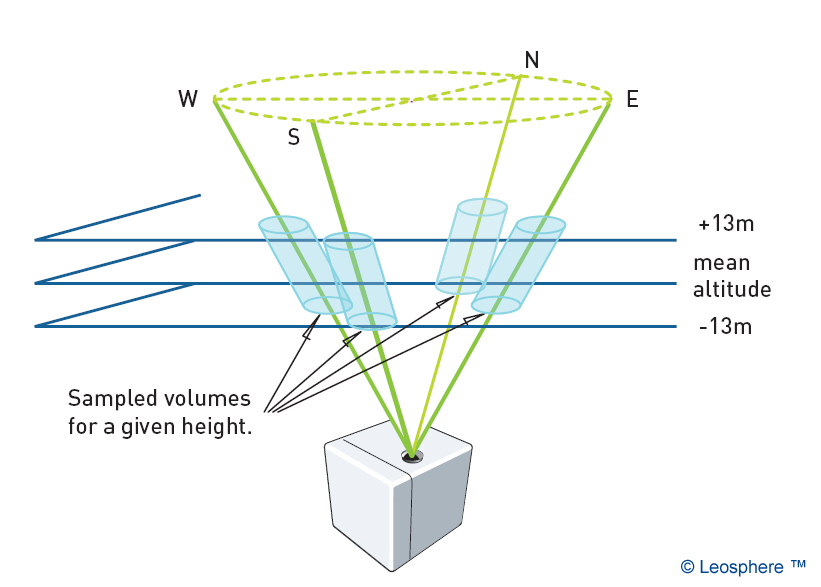
\includegraphics[width=0.9\textwidth]{figures/leosphere_lidar_schematic.jpg}
\caption{Principle of the remote sensing devices’ scanning. Picture shows a Windcube from Leosphere.}
\label{fig:remote_sensing_principle}
\end{figure}

%A comprehensive literature review on Remote sensing for Wind Energy has been compiled by DTU Wind Energy Department after a summer school on the topic. It described the most commonly used instruments and their applicability for wind energy applications [Pena, 2013]. The following descriptions and discussions are based to a large degree on information from this compendium. Additionally, a number of commercially available remote sensing devices have been analysed for the purpose of real-time wind measurement and associated parameters as alternative to met masts. 

%\begin{figure}[h!]
%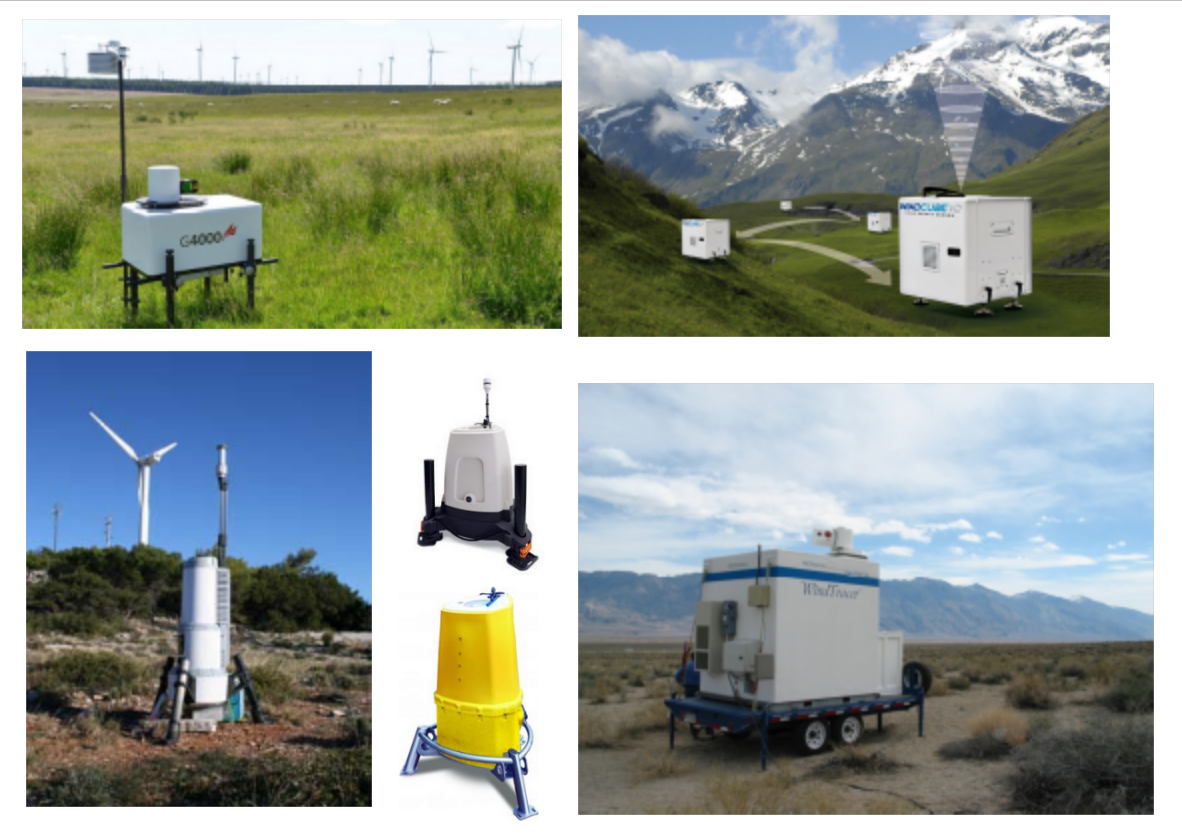
\includegraphics[width=0.9\textwidth]{figures/lidars.png}
%\caption{Examples of LiDARs for wind energy applications. Gallion (left top), Leosphere Windcube (right top), ZephIR (left bottom), ZX300 (mid-bottom upper) Onshore and ZX300M (mid-bottom lower) Offshore Lidars from ZXLidars Zephir ltd. and  Wind Tracer, Doppler LiDAR Lockhead Martin (right bottom).}
%\label{fig:lidars}
%\end{figure}

Ground based remote sensing in wind energy has until recently mostly be driven by a desire to find alternative measurements for expensive and at times difficult installation and erection of met masts. Especially with increasing hub heights, met mast heights have grown to a size, where the erection requires planning permission and cranes of significant size. Hence, it has become so expensive that previously never considered alternatives from the remote sensing area have become price competitive. 

The main driver of recent developments has been the competitiveness in price, the ease of installation and the increasing heights of wind turbines and size of the projects, where it is often no longer sufficient to measure at only one site. Nevertheless, the disadvantage of not directly measuring the target value is still present [W{\"u}rth et al., 2018]. With increasing experience and technical advances in computational science and technology, the remote sensing devices have however become a real alternative.\\

This has also been reflected in the IEC 61400-12:2005 standard, where remote sensing devices have been incorporated as possible devices to carry out wind measurements for wind energy applications in the 2017 update (IEC 61400-12:2017).\\

Looking at the benefits outlined by manufacturers of remote sensing devices (e.g. Sgurr Energy, Vaisala, R-NRG) the following list of key advantages of using remote sensing devices in wind energy applications can be summarised to:\\
\begin{itemize}
    \vspace{-0.2cm}\item Minimal environmental impact
    \vspace{-0.2cm}\item Short installation time
   \vspace{-0.2cm} \item Highly portable
    \vspace{-0.2cm}\item Short lead times
   \vspace{-0.2cm} \item Wind profiling, also above mast height
    \vspace{-0.2cm}\item Measurements over an area or volume
\end{itemize}

The main technical advantage to be considered is the ability to measure over an area or volume rather than at pre-defined fixed heights above the ground. This is also how forecasting models work. NWP models compute variables across grid cells as area averages and area verification of variables are widely applied for model verification in meteorology. 


The drawbacks of remote sensing devices so far have been for both SODAR and LiDAR inaccuracies of signals in complex terrain. According to the white paper of the Deutsche Windguard [2013] and Bradley [2008], especially "in complex terrain sites, influence of the relatively large scanning volume of LiDARs and SODARs must be carefully considered in terms of its influence on the measurement accuracy..". This has been a general observation and a large research topic [see e.g. Bradley, 2012a, Bradley, 2012b, Emeis et al, 2007, Kindler, 2007, Yang, 2013].
Issues and preliminary recommendations of using lidar in complex terrain are summarised by a group from IEA Wind Task 32 in \citep{Clifton2013}. The task also formed a working which is carrying out a group study on several different transfer methods for the use of lidar in complex terrain. Results are expexted in 2021. 

Although LiDARs and SODARS, as well as RADARS and wind profilers have quite a long tradition to be used in measuring campaigns in atmospheric science, data assimilation and numerical modelling (e.g. [Wilzcak et al, 1995, Grund et al., 2001, Benjamin et al., 2004, Pichugina et al, 2008]), these instruments have been prone to measurement uncertainty and require special treatment and verification algorithms, if they are used in real-time applications. 

%\begin{figure}[h!]
%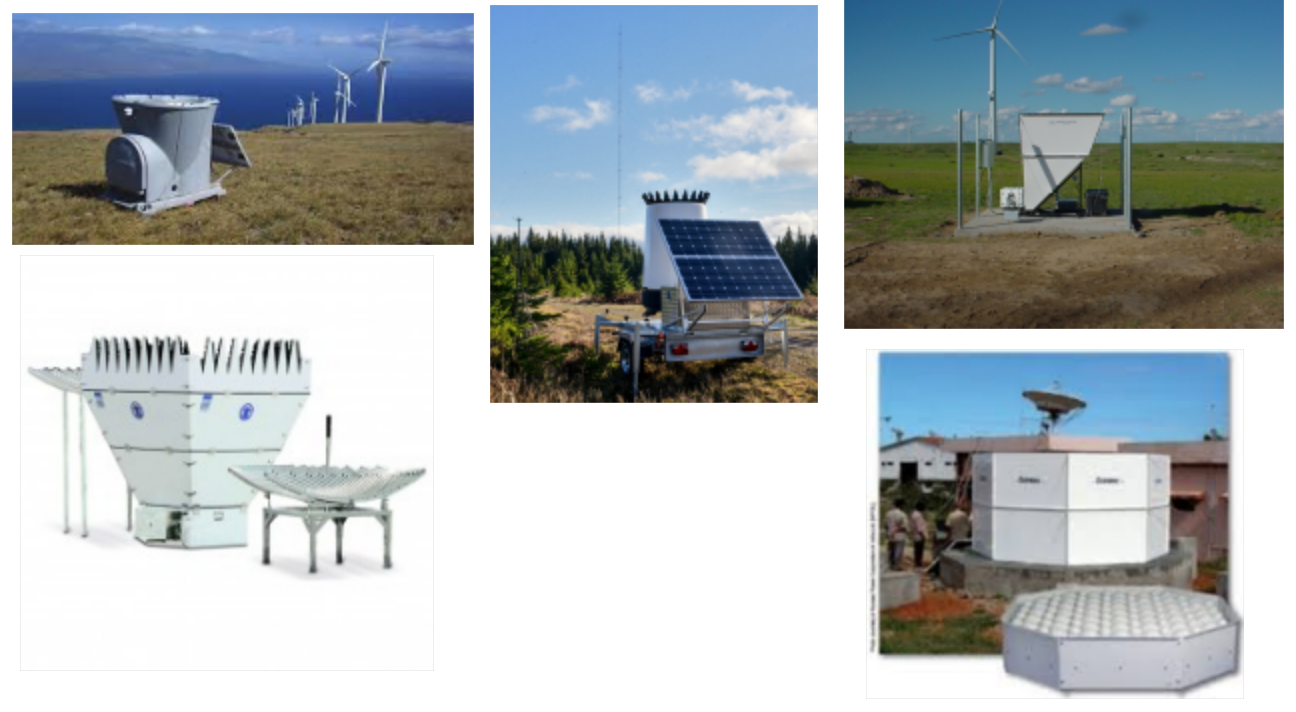
\includegraphics[width=0.9\textwidth]{figures/sodars.png}
%\caption{Examples of SODARs used in wind energy applications. Vaisala Triton (left top), AQ 510 , (middle top), ASC 4000i (top right), METEK PSC (bottom left), Scintec XFAS (bottom right).}
%\label{fig:sodars}
%\end{figure}

There has been a rapid development in LiDAR and SODAR technology over the past 10 years. Figure 4 and Figure 5 show the most common used devices in the context of wind energy projects and studies. While in the years up to 2013 most field studies spoke about the Remote Sensing devices such as SODAR and LiDAR as promising for site assessment [e.g. Kelley et al., 2007, Mann et al., 2008, Bradley et al., 2008, Bradley et al., 2012, Pena et al., 2013, Lang and McKeogh, 2013], it was only in 2013 that the first SODAR was classified for the IEC 64100-12 standard of site assessment and the ZEPHIR LiDAR was assessed and validated against a IEC compliant mast in a demonstration with a sample size of more than 170 verification cycles at UK’s Remote Sensing Test Site.\\ 

ZEPHIR LiDAR's white paper [Burin des Roziers, 2014] states that the Zephir LiDAR proves that it ".. delivers LiDAR systems well within the IEC criteria for wind  measurement  equipment. The  evidence  is gathered  across  the  largest single-type batch  of  LiDAR performance  validations against  an IEC compliant mast."

The common findings of all the experimental measuring campaigns as well as real-time testing is that the instruments need to be well serviced and are maintained similar to any other real-time instrument operating under changing conditions throughout the yearly cycles. 
If this is not done, echoes, interfering noise sources, laser beam disturbances deteriorate the instruments and make the further processing of the data impossible. 
It is also commonly understood that it requires skilled personnel to install and maintain such instrumentation, if it should run continuously and reliably. For a real-time application it is additionally crucial that the measurement signals can be used as is and need no further processing.


%\subsubsection{Remote sensing devices for wind farms in complex terrain} \label{sec:remote_sensing_in_complex_terrain}

%It has been reported in several studies [Bradley, 2008b, 2012a, 2012b, Bingöl, 2009a, 2009b], that the difficulty of the installation of met masts in complex terrain sets a burden on projects. SODARs and LiDARs are much faster and easier to install, since they usually ship as a self contained unit, and can be easily assembled. These advantages from a practical and economic perspective are well known. The disadvantages that are reported are the difficulties LiDARs and SODARs have in replicating correct wind speeds in complex terrain. One of the issues is that the light conus is disturbed by the changing terrain. If this is the case, independent of whether this is an acoustic or light signal, the measurements are no longer correct and are mostly underestimated. In a study carried out in complex terrain in Bosnien-Herzegowina [Wagner, 2014], this discrepancy was 4.5\% in comparison to a mast. However, Leosphere, one of the LiDAR manufacturer equipped the instruments with a so-called "Flow Complexity Recognition" (FCR) feature that corrected the signals in the signal processing step for the underestimation. With this FCR algorithm applied, the results were in reasonable agreement with the mast and within the expected uncertainty range. Another issue that has been reported in real-time operation of remote sensing devices are measurement problems after lightning. These devices are more prone to lightning strikes, which means that for long-term operation this topic needs to be taken into account as part of the technical requirements, especially in areas, where lightning is a common weather phenomenon. The manufacturers are obviously aware of the issues and are most likely working on protection systems. Therefore, this is not considered problematic, however lightning protection and recovery strategies after lightning should be part of the technical requirements of these instruments.


Today's available remote sensing devices seem to suggest that the instruments are at a development stage, which makes them interesting for real-time forecasting and grid operation purposes. However, there are quite a number of technical requirements that need to be present to ensure data collection of a quality necessary for the use in real-time forecasting for grid operators.\\ 

{\color{red}{Comment COM 21.08.2021: Is this the right place for this recommendation ?\\}Summary of the recommended technical requirements to ensure high quality data in long-term real-time operation:
\begin{itemize}
    \vspace{-0.2cm}\item measurements must be raw or technical requirements must include maintenance and software updates
    \vspace{-0.2cm}\item lightning protection and recovery strategy after lightning
measurements should be taken at a height appropriate for the wind farm, either at one of preferable at both hub height and around 30m
    \vspace{-0.2cm}\item instruments must be serviced and maintained by skilled staff
    \vspace{-0.2cm}\item version control must be maintained for signal processing
    \vspace{-0.2cm}\item wind characteristics data must be on wind turbine level
    \vspace{-0.2cm}\item LiDARs and SODARs in complex terrain require special consideration 
\end{itemize}
}

%\section{Instrumentation on Met stations }\label{sec:metstations}
\subsection{Nacelle instrumentation and measurements{\color{blue}{ -- needs attention}}}\label{sec:Nacelle measurements}

Among the nacelle measurement devices there are three types that are commonly used:
\begin{itemize}
    \item cup anemometers
    \item horizontally mounted LiDAR (Wind Iris, ZephIR)
    \item (ultra-) sonic anemometers (iSpin technology, ROMOWIND)
\end{itemize}


\begin{figure}[h!]
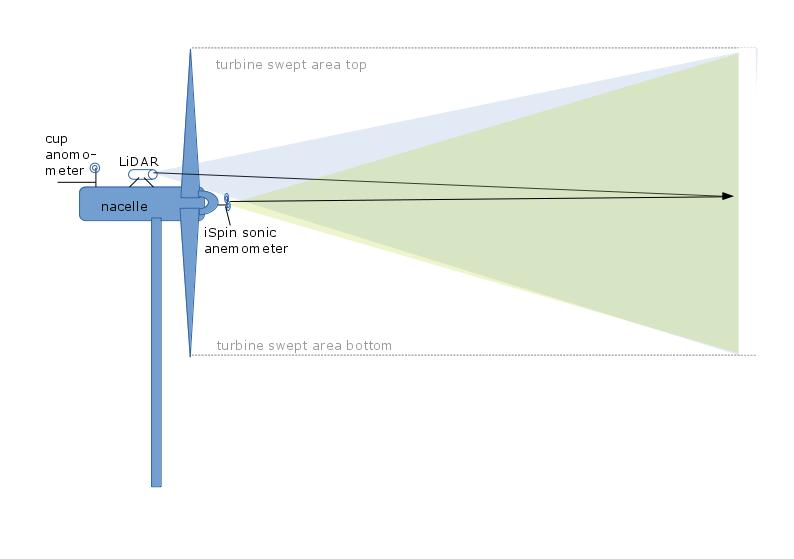
\includegraphics[width=0.9\textwidth]{figures/nacelle_mounted_instruments.jpg}
\caption{Schematic of the nacelle mounted instruments cup anemometer, LiDAR and iSpin ultra-sonic anemometer. The latter two instruments look forward into the wind eye and cover the rotor swept area.}
\label{fig:nacelle_schematic}
\end{figure}

.\\
Figure \ref{fig:nacelle_schematic} shows a schematic of the instruments and how and where they are mounted at the turbine’s nacelle. The cup anemometers are typically mounted at the back of the nacelle. The horizontally mounted LiDAR is mounted approximately in the middle of the nacelle with a slight displaced angle in order to cover the total swept area of the rotor in the direction of the eye of the wind. The iSpin ultra-sonic anemometers are mounted at the front of the nacelle, looking kind of undisturbed into the eye of the wind. 


\subsection{Cup anemometers}\label{sec:cup_anemometers}

Most commonly cup anemometers with wind vanes for direction measurements are installed at the nacelle. There are the IEC 61400-12-1, the 61400-12-2 and the ISO/IEC 17025 standards that describe how these instruments must be calibrated and mounted as well as describing the process and the integrity of the measurement processes and design of the mast, instruments and measuring procedures. This will also be discussed in the standard’s analysis in Section \ref{ch:reference_to_applicable_standards}. In this section, we only discuss, whether and how the data from cup anemometer instrumentation at the nacelle can add value to forecasting.\\
The cup anemometers at the nacelle have one distinctive advantage over any other instruments: they are installed at the turbine and connected to the SCADA system that is delivering data to the system operator. HOwever, this advantage comes with a downside: the measurements taken at the nacelle are affected by two major disturbances: (1) the rotating turbine blades, which generates so-called yaw-misalignment and (2) wake effects from other wind turbines in the direction of the wind. In the worst collection hours both phenomena disturb the signal of the nacelle instrument and the signals can cause deterioration of the forecast, if they are used in the data assimilation phase.

\begin{figure}[h!]
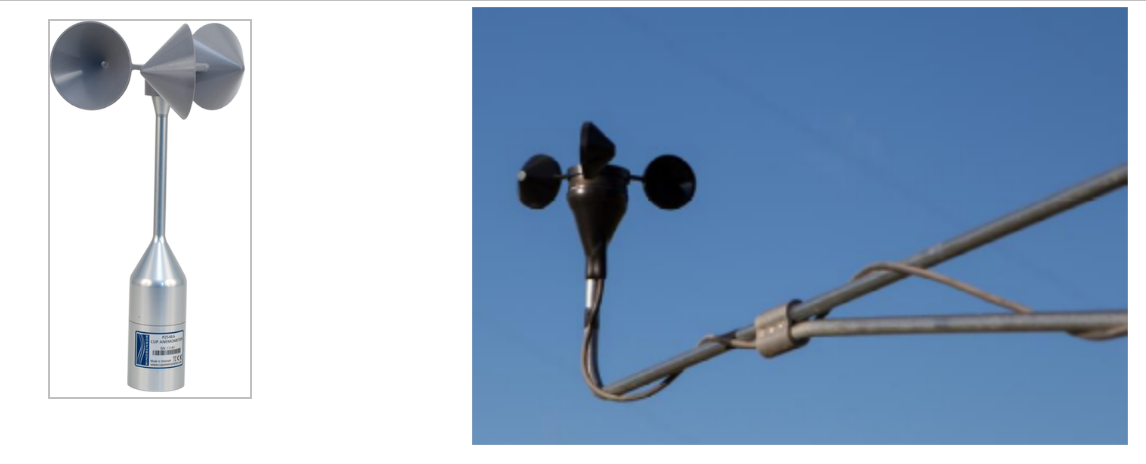
\includegraphics[width=0.9\textwidth]{figures/anemometer_cup.png}
\vspace{-0.2cm}\caption{MEASNET certified cup anemometer from Cambell Scientific and a cup anemometer 40C from RNRG.}
\label{fig:measnet_cup_anemometers}
\end{figure}


\subsection{Sonic and ultra-sonic anemometers}
The sonic and ultra-sonic 3D anemometers have a long tradition in atmospheric science and meteorology in relation to boundary layer studies of turbulence intensity and phenomena like low level jets. These instruments are well tested and can be used for real-time operations, but are mostly considered too expensive for traditional wind measurements [e.g. Berg  et al. 2012, Popinet et al., 2006, Basu et al., 2004, Lundquist, 2014]. 

\begin{figure}[h!]
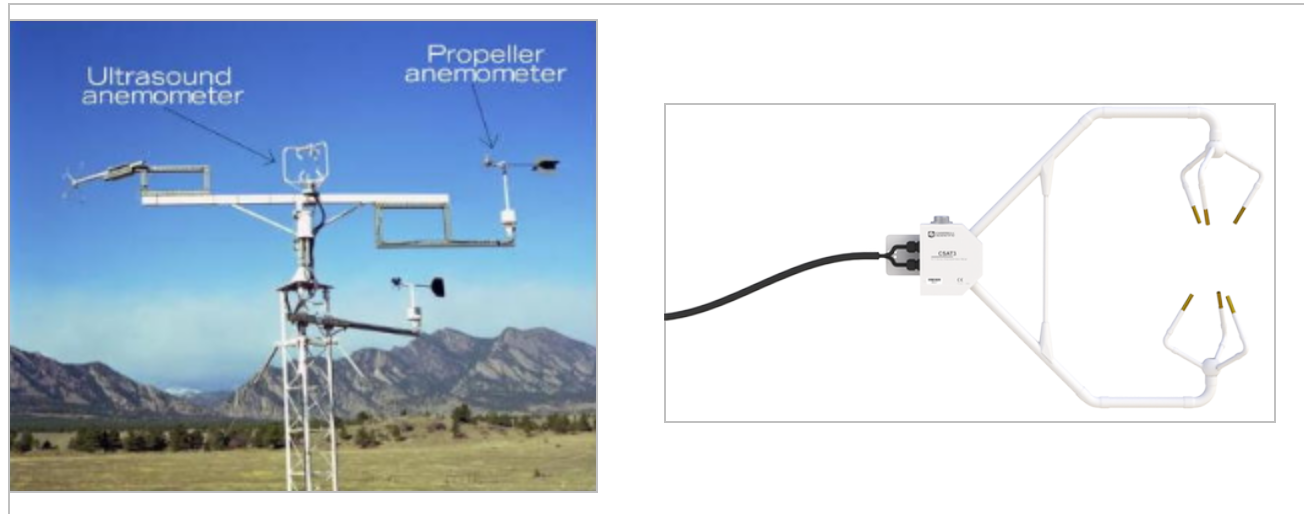
\includegraphics[width=0.9\textwidth]{figures/anemometer_sonic.png}
\caption{Example of a 3D ultra sonic anemometer and a propel anemometer at the NREL test site in Colorado (left) and a 3D sonic anemometer from Campbell scientific (right).}
\label{fig:nrel_sonic_anemometers}
\end{figure}

Figure \ref{fig:nrel_sonic_anemometers} shows a mast with an ultra-sonic anemometer at the NREL test site in Golden, Colorado and a well-tested 3D sonic anemometer from Campbell Scientific.\\

A newer type of sonic anemometer are the so-called ultra-sonic 3D spinner anemometer instruments, short “iSpin”, which have found their way into instrumentation for wind energy. Figure \ref{fig:nrel_sonic_anemometers} shows the principle of the iSpin anemometer from ROMOWind and an installed spinner anemometer example from METEK. With the update of the IEC standard 61400-12-2, the iSpin technology has become part of the measurement types to define the absolute power curve. The iSpin technology strictly speaking are sonic anemometers that are mounted at the tip of the nacelle, in front of the turbine blades, looking forward in wind direction and rotating with the blades. This means that the velocity of the rotating blades is taken into the computation of the signals and wake effects and yaw misalignment from the blades are measured instead of the signal being disturbed by the rotating blades. 

There are a number of studies that have been carried out since 2011, when the instruments were first launched by ROMO Wind. A review made by GL-Garrad Hassan [Falbe-Hansen, 2012] and DNV-GL [DNV-GL, 2015] provide a comprehensive overview of the technology and it's development from 2011 to today. 

\begin{figure}[h!]
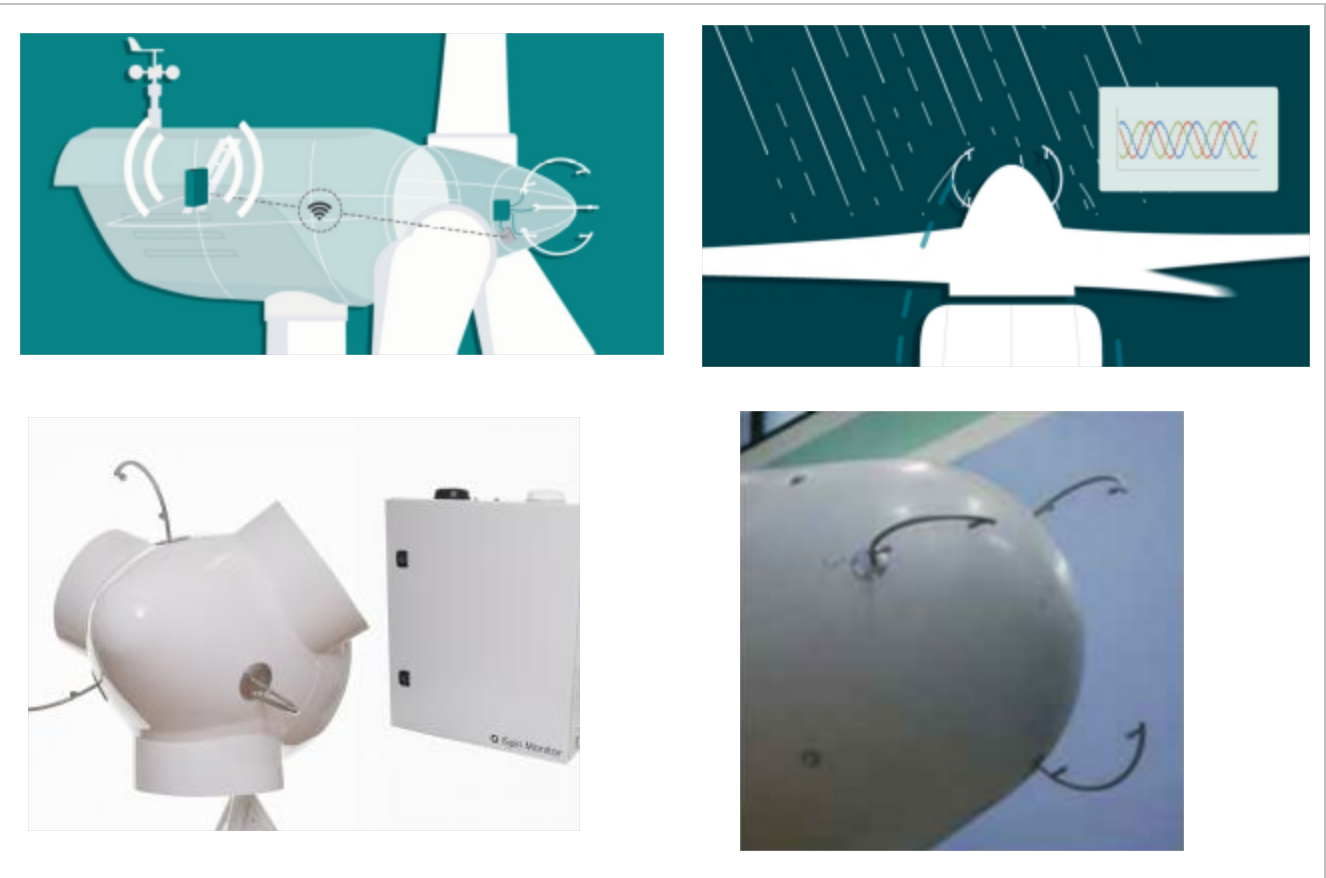
\includegraphics[width=0.9\textwidth]{figures/nacelle_ispinner.png}
\caption{Ultra-sonic anemometer spinner technology iSpin from ROMO Wind as schematic and also an example of a nacelle top mounted from METEK (bottom right).}
\label{fig:ispinner}
\end{figure}

DTU Wind (Risø) has published some documents describing the technology characteristics and basic principles [Pedersen et al., 2007, 2016]. The so-called spinner ultra-sonic 3D anemometer technology “iSpin” has been installed in 2016 on a large fleet of wind turbines in Denmark. The turbines are operated by Vattenfall and the iSpin devices are delivered, implemented and maintained by ROMOWIND [ROMOWIND, 2016]. Unfortunately there are currently no publications available regarding real-time experience. From personal communication with Vattenfall research department, it can however be stated that the results look promising regarding the fit of wind measurements to the power production. 

ROMOWIND provides free access to data collected with their iSpinners at the Nørrekær Enge wind farm in Denmark, which was commissioned in 2009 and consists of 13 Siemens SWT 2.3-93 wind turbines at 80 m hub height [ROMO WIND, 2016].\\ With this, ROMOWIND and Vattenfall (the owner of the wind farm) provide the opportunity to experts and researchers to carry out experiments and studies with the data from the 3D-spinners and compare these data to a met mast and other nacelle mounted cup anemometers.
The open-access project is supported by the Danish EUDP program and data was collected under this program from 1st November 2014 to 17th December 2015. 
This might be a good opportunity to study the performance and the costs in a real environment and thereby be able to provide recommendations regarding the applicability of this technology in the context of forecasting.


\subsection{Horizontally mounted nacelle LiDAR}
{\color{blue}{needs attention - more authors: IW/AC ?}}

Another nacelle mounted wind measurement device is a horizontally mounted LiDAR at the turbine nacelle. Theoretically, every LiDAR can be mounted in that way. However, the space and requirements on top of the wind turbine are very different to the ground. Hence, there is only one commercially available instrument on the market at present, the “Wind Iris LiDAR” from Renewable-NRG [Morton, 2016]. Nevertheless, we will analyse some of the studies carried out with other devices (e.g. ZePHIR LiDAR) to investigate it's applicability in the context of forecasting and system operation. Strictly speaking this device belongs to the remote sensing devices. Nevertheless, it is a horizontally mounted LiDAR at the nacelle that looks towards the wind eye and has the same characteristics as the iSpin ultra-sonic anemometers, but is typically mounted at the back of the nacelle similar to the classical cup anemometer. 
Because it is mounted at the nacelle and is measuring the wind in a conus towards the wind eye, the Wind Iris can measure a kind of profile throughout the sweep area of the rotor. This makes the instrument to an interesting device not only for performance measurements, but also for forecasting.

\begin{figure}[h!]
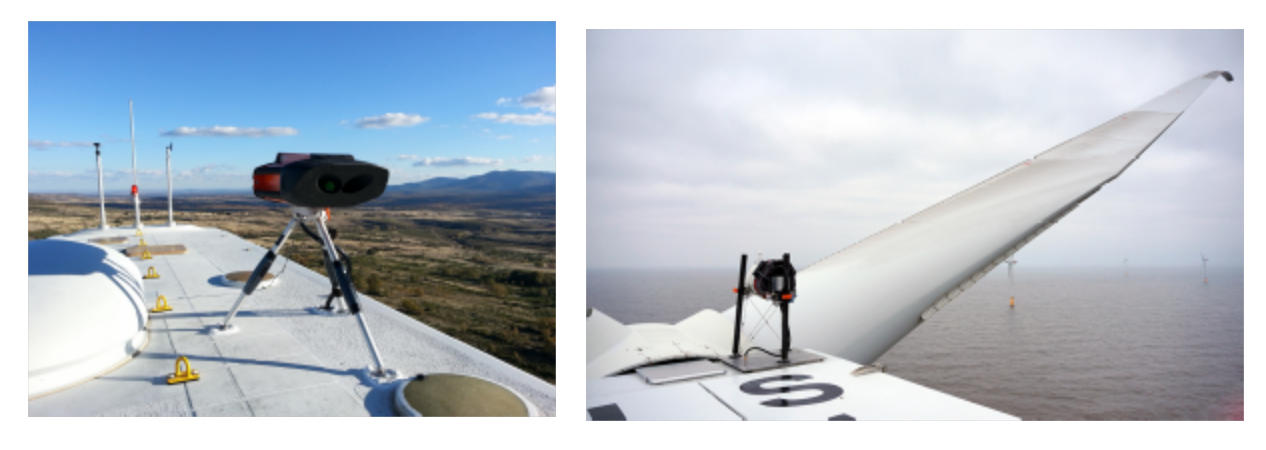
\includegraphics[width=0.9\textwidth]{figures/nacelle_lidar.png}
\caption{Example of nacelle mounted METEK iSpin technology and ZephIR ZXTM LiDAR.}
\label{fig:ispinner}
\end{figure}


Angelou et al. [2010] compared a sonic anemometer and a ZePHIR LiDAR mounted at a V27 Vestas turbine at the same height. He found out that the precision of the LiDAR in detecting fast fluctuations of the wind speed was not as high as for the sonic anemometer at the met mast. However, the authors concluded that for applications, where 10 min averages are of high enough time resolution this isn't a problem. In their experiment, the direction measurement however "ran off" and caused a decrease in wind speeds in comparison to the mast mounted sonic. 

Today, Zephir Ltd. provides the ZXTM Lidar commercially, where it compensates for turbine movement automatically and it's said that the data can be used for the standard industry methodologies and measurements for power curves, nacelle transfer function calibration including yaw alignment, and Wake detection (ZXLidars product specification \url{https://www.zxlidars.com/wp-content/uploads/2021/02/ZX_Lidars_ZX-TM-Summary_05022021_digital.pdf}.\\



\section{Instrumentation for Solar Projects}\label{sec:solar_instrumentation} 
%\section{Sensors for solar energy {\color{blue}{needs attention/AK, SW, MF}}}\label{sec:solarradiation}
{\color{blue}{Contributing authors: SW -- status ?}}

% diagram of instruments (sky-imager, satellite, NWP)

The following is a list of parameters and instruments that are typically installed on solar power plants to monitor the plant's performance and/or to use the data for forecasting applications according to the application and the type of PV system. 


\begin{itemize}
    \item ground-mounted PV systems 
\begin{itemize}
    \item Parameter: Global Horizontal Irradiation (GHI), includes both Direct Normal Irradiation (DNI) and Diffuse Horizontal Irradiation (DHI),  Global Tilted Irradiation (GTI)
    \item Instruments: 
        \begin{itemize}
            \item Pyranometer (horizontal (GHI), tilted (GTI), with shadow ball or shadow ring (DHI)
            \item Pyrheliometer (DNI)
            \item  Reference cell (GHI)
        \end{itemize}

\end{itemize}
    \item ground-mounted tracking PV systems 
        \begin{itemize}
            \item Parameter: 
            \item Instruments: 
            \begin{itemize}
                \item Pyranometer (horizontal (GHI), tilted (GTI))
                \item Pyrheliometer installed on a sun tracker (DNI, DHI)
                \item Rotating Shadowband Irradiometer (DNI, DHI)
            \end{itemize}
        \end{itemize}

    \item Concentrated PV
        \begin{itemize}
            \item Parameter: 
            \item Instruments: 
            \begin{itemize}
                \item Pyranometer (horizontal (GHI), tilted (GTI))
                \item Pyrheliometer installed on a sun tracker (DNI, DHI)
            \item Rotating Shadowband Irradiometer (DNI, DHI)
            \end{itemize}
        \end{itemize}
    \item Large-scale Roof-top PV
        \begin{itemize}
        \item Parameter: 
        \item Instruments: 
            \begin{itemize}
                \item Pyranometer (horizontal (GHI), tiltet (GTI))
                \item Pyrheliometer installed on a sun tracker (DNI, DHI)
            \end{itemize}
        \end{itemize}
\end{itemize}

Note, small scale roof-top systems for households are not considered here, as these systems are too small for specific or additional meteorological measurements.

In the ``Best Practices Handbook  for the Collection and Use  of Solar Resource Data for Solar Energy Applications'' (referred to also as ``PVPS handbook'') \cite{nrelhandbook2021} the following other meteorological measurements are mentioned: 

\begin{itemize}
    \item Met Stations:
        \begin{itemize}
            \item Wind Speed anemometers
            \item Ambient Temperature and Relative Humidity sensors
            \item Atmospheric Pressure sensor
            \item Precipitation sensor or gauge
            \item Aerosols and Water Vapor ???
        \end{itemize}
   \item Spectral Irradiance 
   \item Ultraviolet Irradiance 
   \item Soiling sensors
   \item All sky imagers
   \item Circumsolar Radiation 
   \item Beam Attenuation Between Heliostats and Receiver in Tower Power Plants
   \item Surface Albedo measurement/calculation: 
         \begin{itemize}
            \item round measurements using albedometers (two pyranometers placed horizontally in opposite up and down directions, measuring GHI and RHI, respectively)
            \item satellite estimates based on monitoring the reflected radiance emanating from the Earth’s surface-atmosphere system
            \item predictions based on a reanalysis model
        \end{itemize}
\end{itemize}

These instrumentations will be described in more detail in the following sections. 

\subsection{Point Measurements }

  Pyranometer, incl. albedometers, shaded pyranometers, 
  Reference cell
  Pyrheliometer on sun tracker
  em Rotating Shadowband Irradiometer
Sunshine Duration Sensor
soiling measurements 

For  concentrating systems the measurement of circumsolar radiation can be beneficial. This can be done with rotating shadowband irradiometers, pyrheliometers with different acceptance angles or special camera systems. For solar tower plants furtehr measurements are of interest to provide information on the beam attenuation between the mirrors and the receiver.

The further instrumentation for point measurements with anemometers, temperature sensors, pressure sensors, hygrometer sensors and precipitation sensors has bee described above related to met masts

 
\subsection{Sky-imaging}

\subsection{Satellite Data}




%\iffalse
%\section{Power Measurement Systems}\label{sec:scadasystems}
%
%\subsection{Energy Meters}
%
%Energy meters at connection point as used in settlement and live feed to System Operators. Distinct from plant SCADA.
%
%\subsection{Wind Power SCADA systems {\color{magenta}{Contributing author: JB}}}\label{subsec:scadasolar}
%
%Suggested content:
%\begin{itemize}
 %   \item Turbine anemometer (and issues)
  %  \item Relevant turbine parameters
   % \item Relevant derived quantities (e.g. rotor effective wind speed, power available)
%    \item ???
%\end{itemize}

%\subsection{Solar Power SCADA Systems {\color{magenta}{Contributing author: ?}}}\label{subsec:scadawind}
%fi

%\section{}\label{sec:}

%\subsection{}\label{subsec:}
